\chapter{Microservices}

The scalability dimension of software architecture can be represented by the following figure:

\begin{figure}[h!]
  \centering
  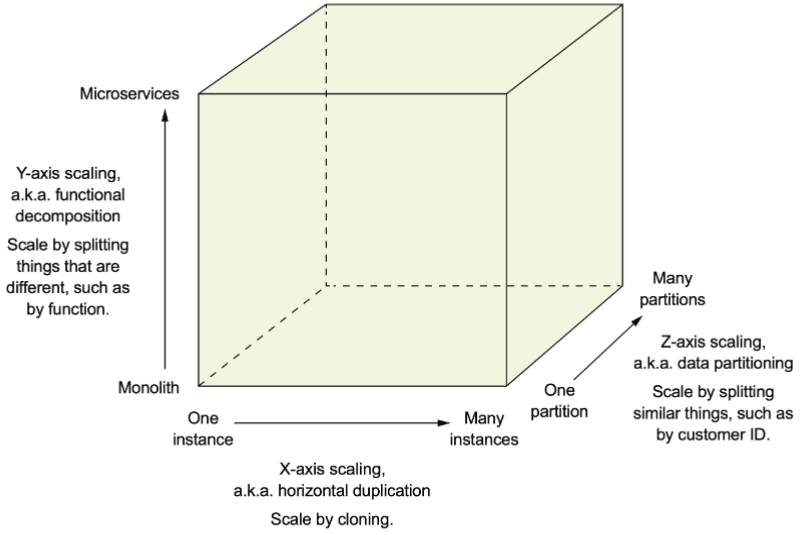
\includegraphics[width=0.35\linewidth]{content/chapters/images/2026-04-11-11-42-08.png}
\end{figure}


\begin{table}[h!]
  \renewcommand{\arraystretch}{1.6}
  \centering
  \begin{tabularx}{0.8\textwidth}{X X}
    \toprule
    \textbf{Advantages}                                        & \textbf{Disadvantages}                                                                      \\
    \midrule
    Enables the continuous delivery and
    deployment of large, complex applications                  & Finding the right set of services is challenging                                            \\
    Services are small and easily maintained                   & Distributed systems are complex, which makes development, testing, and deployment difficult \\
    Services are independently deployable                      & Deploying features that span multiple services requires careful coordination                \\
    Services are independently scalable                        & Deciding when to adopt the microservice architecture is difficult                           \\
    Enables teams to be autonomous                             &                                                                                             \\
    Allows easy experimenting and adoption of new technologies &                                                                                             \\
    Better fault isolation.                                    &                                                                                             \\
    \bottomrule
  \end{tabularx}
\end{table}


\begin{figure}[h!]
  \centering
  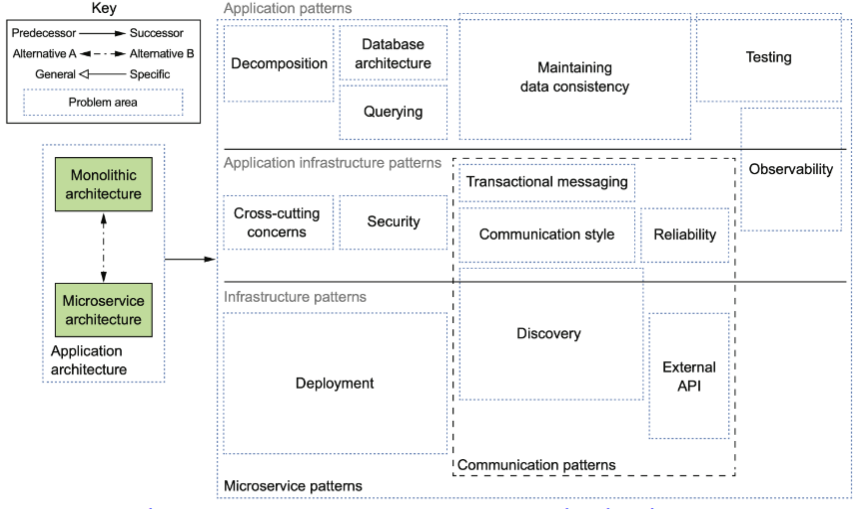
\includegraphics[width=0.75\linewidth]{content/chapters/images/2026-04-11-12-18-32.png}
\end{figure}

\subsection{Monolith vs. Microservices}




\begin{flushleft}
  \begin{minipage}{0.65\linewidth}
    \raggedright
    The problem is the deployment in fact:

    \begin{itemize}
      \item Monolithic architecture: Simple to develop, deploy, and scale.
      \item Microservices architecture: Simple to mantain, to test and flexible to scale
    \end{itemize}
  \end{minipage}%
  \hfill
  \begin{minipage}{0.3\linewidth}
    \centering
    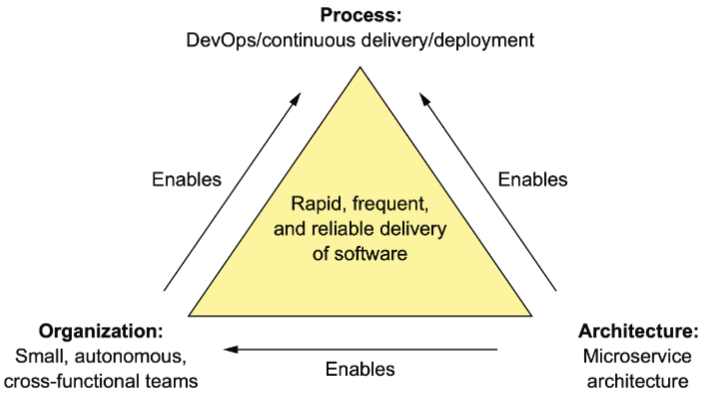
\includegraphics[width=\linewidth]{content/chapters/images/2026-04-11-12-21-52.png}
  \end{minipage}
\end{flushleft}


\subsection{Decomposition}



\begin{flushleft}
  \begin{minipage}{0.65\linewidth}
    \raggedright
    Decomposition identifies system operations:

    \begin{itemize}
      \item Understand domain model
      \item Define operations
      \item  Identify use cases
    \end{itemize}

    and decompose the system into subsystems or subdomains.

  \end{minipage}%
  \hfill
  \begin{minipage}{0.3\linewidth}
    \centering
    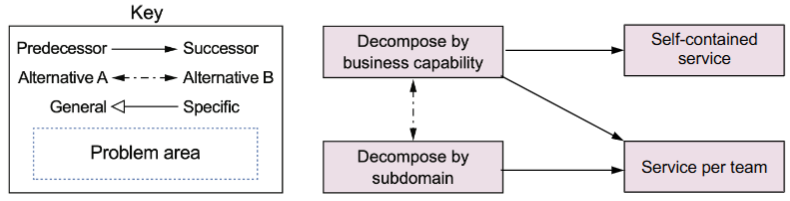
\includegraphics[width=\linewidth]{content/chapters/images/2026-04-11-12-22-47.png}
  \end{minipage}
\end{flushleft}

\paragraph{Domain model Example}

\begin{figure}[h!]
  \centering
  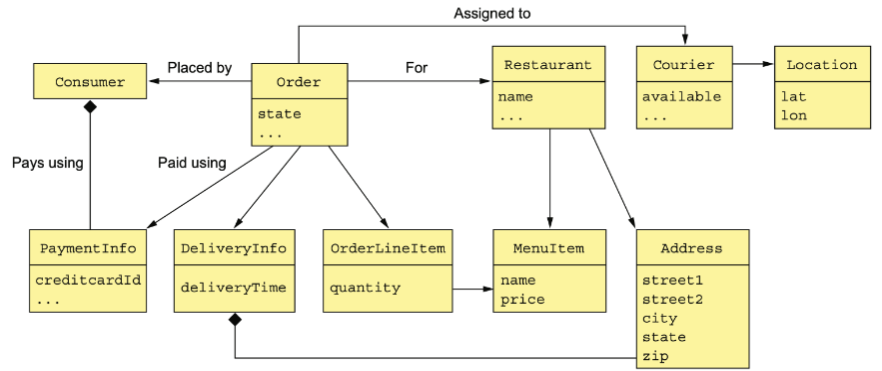
\includegraphics[width=0.4\linewidth]{content/chapters/images/2026-04-11-12-26-07.png}
\end{figure}

\subsubsection{User stories}

\begin{table}[h!]
  \renewcommand{\arraystretch}{1.6}
  \centering
  \begin{tabular}{l l l}
    \toprule
    \textbf{Actor}   & \textbf{Goal}   & \textbf{Services} \\
    \midrule
    Consumer         & Create order    & Order             \\
    Restaurant       & Accept order    & Order             \\
    Restaurant       & Complete order  & Kitchen           \\
    Courier          & Update location & Delivery          \\
    Courier          & Pick up         & Delivery          \\
    Courier          & Delivery        & Delivery          \\
    Delivery company & Manage couriers & Courier           \\
    Delivery company & Courier payment & Accounting        \\
    \bottomrule
  \end{tabular}
\end{table}



\subsubsection{By business capability}

\begin{enumerate}
  \item An organization business capability is what it does (as opposed to how). Look into organization structure, also consistent operations, stories or goals.
  \item Single Responsibility Principle
  \item Common Closure Principle - classes that change for the same reason should be in the same package
  \item Result is cohesive and loosely coupled
\end{enumerate}

\subsubsection{By subdomain}

\begin{flushleft}
  \begin{minipage}{0.65\linewidth}
    \raggedright
    \begin{itemize}
      \item Identify bounded contexts - DDD sub-domains. Partitions of overall domain model
      \item Result is cohesive, Loosely coupled, allow cross-functional and
            autonomous teams and scalable architecture
    \end{itemize}

  \end{minipage}%
  \hfill
  \begin{minipage}{0.3\linewidth}
    \centering
    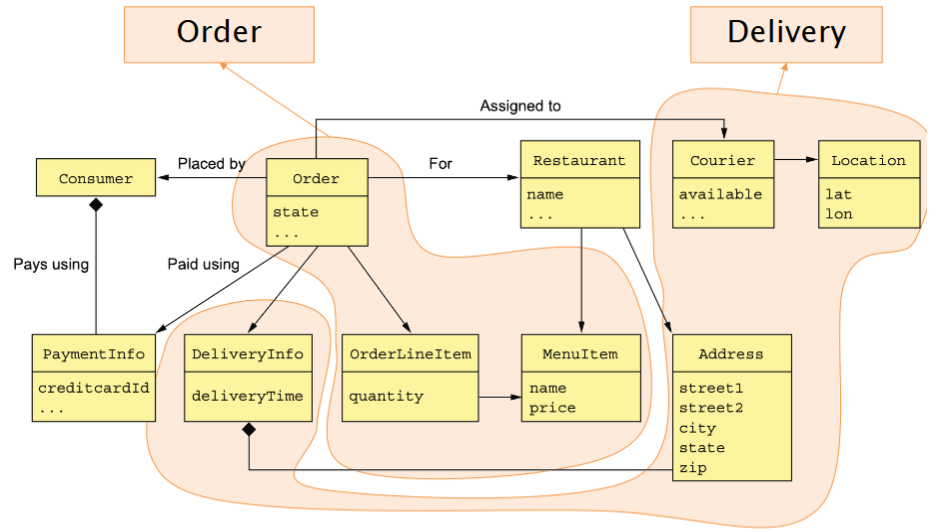
\includegraphics[width=\linewidth]{content/chapters/images/2026-04-11-12-34-15.png}
  \end{minipage}
\end{flushleft}

\subsection{Guidelines from OOP}

\paragraph{Single Responsibility Principle} - A class should have only one reason to change.
\paragraph{Common Closure Principle} - The classes in a package should be closed
together against the same kinds of changes. A change that affects a package
affects all the classes in that package.

\subsubsection{Decomposition obstacles}
\begin{itemize}
  \item Network latency
  \item Reduced availability due to synchronous communication
  \item Data consistency across services
  \item Obtaining a consistent view of the data
  \item Good classes
\end{itemize}


\section{Business logic}

\begin{figure}[h!]
  \centering
  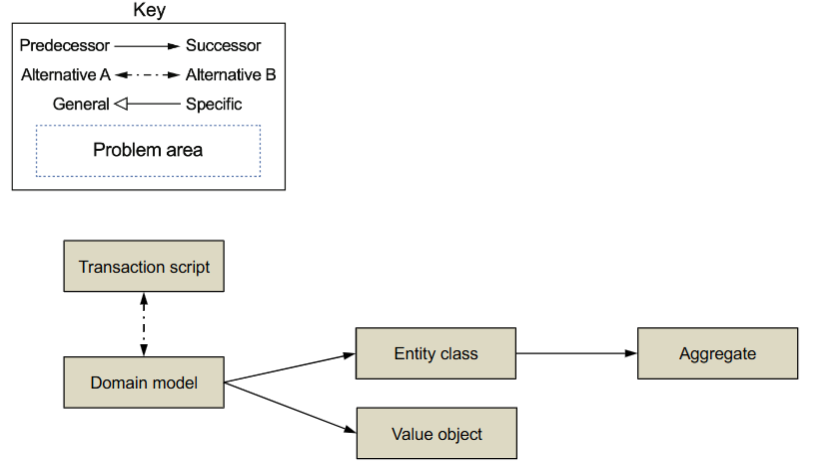
\includegraphics[width=0.4\linewidth]{content/chapters/images/2026-04-11-12-45-11.png}
\end{figure}

\subsection{Transaction script}
When you have simple business logic that
consist of a sequence of steps.


Organize business logic by procedures
where each procedure handles a single
request from the presentation.

One service class with a method for each procedure. Several data classes.

Consequences:

\begin{itemize}
  \item All the code for a request in a single place
  \item Code duplication for similar requests
  \item Difficult to maintain and refactor
\end{itemize}


\subsection{Domain model}
When you have complex business logic

Adopt recommended object-oriented
methods to create classes that encapsulate
both code and data, using the DDD approach.

Consequences:

\begin{itemize}
  \item Code for a request is spread among classes
  \item No code duplication
  \item Easy to maintain and refactor
  \item Easy to extend with Strategy or Template Method patterns
\end{itemize}

\subsection{Ports \& Adapters (hex)}


\begin{figure}[h!]
  \centering
  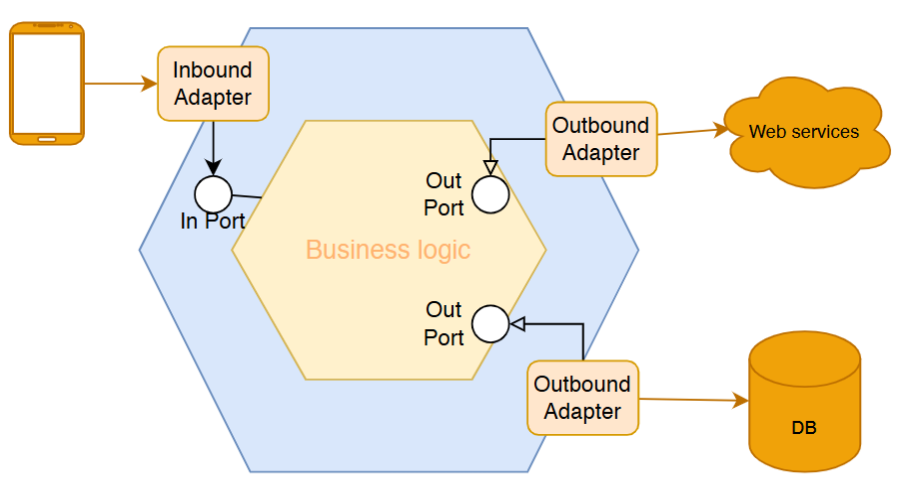
\includegraphics[width=0.4\linewidth]{content/chapters/images/2026-04-11-12-46-25.png}
\end{figure}


\section{Domain Driven Design - DDD}


\begin{itemize}
  \item Sub-domains
  \item Bounded context
  \item Class types patterns: Entity, Value Object, Service, Repository, Factory
  \item Aggregate
\end{itemize}

\subsection{Sub-Domain \& Bounded Context}
DDD decompose the overall domain
model into sub-domains. Each sub-domain is valid within a
bounded-contex.


A bounded-context brings together a common language and people, team, focusing on a shared problem.
Distinct contexts are related to each
other in order to enable communication.

\subsection{Class patterns}

\begin{itemize}
  \item Entity - Represents objects that have a persistent identity. Two
        objects with the same values represent distinct items. Usually, they are
        persisted to a db
  \item Value object - Represents a collection of values. Two objects with the same values are
        interchangeable
  \item Factory - Implement object creation logic. May hide concrete class
  \item Repository - Provides access to persistent entities. Hides access to db
  \item Service - Implements business logic that does not belong to a single entity
\end{itemize}

\subsection{Domain boundaries}

Often domain models have fuzzy
boundaries. All strictly related concepts should
belong to the same context. E.g. \verb|Order| and \verb|OrderLineItem| classes.

Not keeping together such classes might
result in violations of business rules or
invariants, upon updates. E.g. minimum amount for an order.

\begin{figure}[h!]
  \centering
  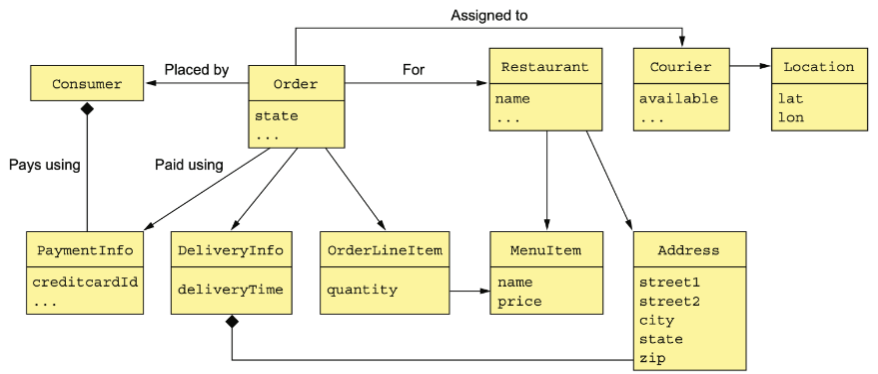
\includegraphics[width=0.4\linewidth]{content/chapters/images/2026-04-11-12-56-55.png}
\end{figure}


\subsection{Aggregate pattern}
Organize a domain model as a collection
of aggregates, each of which is a graph
of objects that can be treated as a unit.

Decompose domain model into chunks:

\begin{itemize}
  \item Self contained units
  \item Easier to understand
  \item Clarify scope of operations
  \item All elements share the same life cycle
\end{itemize}

\begin{figure}[h!]
  \centering
  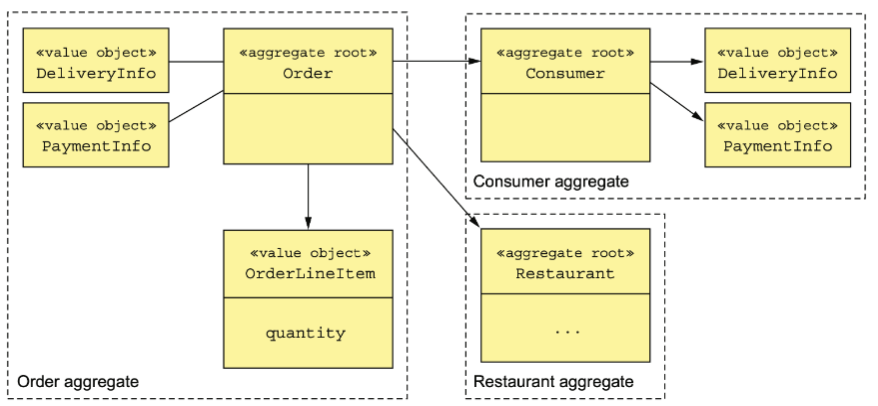
\includegraphics[width=0.4\linewidth]{content/chapters/images/2026-04-11-12-58-44.png}
\end{figure}

\subsection{Rule: reference roots only}

Reference only the aggregate root. Updates go through methods of aggregate root.
When a repository loads an aggregate from the db it returns a reference to the
aggregate root.

Consequences:

\begin{itemize}
  \item Enable aggregate to enforce consistency rules
  \item Aggregate updates are serialized
\end{itemize}


\begin{flushleft}
  \begin{minipage}{0.65\linewidth}
    \raggedright
    \subsection{Rule: primary keys inter aggregate}
    Inter-aggregate references \textbf{must use
      primary keys}. NOT using object reference, indeed, this is usually code smell.

    Consequences:
    \begin{itemize}
      \item Loose coupling of aggregates
      \item Keep aggregate boundaries enforced
      \item Avoid accidental cross-aggregate updates
      \item Aggregates can belong to distinct services
      \item Simplify persistence
    \end{itemize}
  \end{minipage}%
  \hfill
  \begin{minipage}{0.3\linewidth}
    \centering
    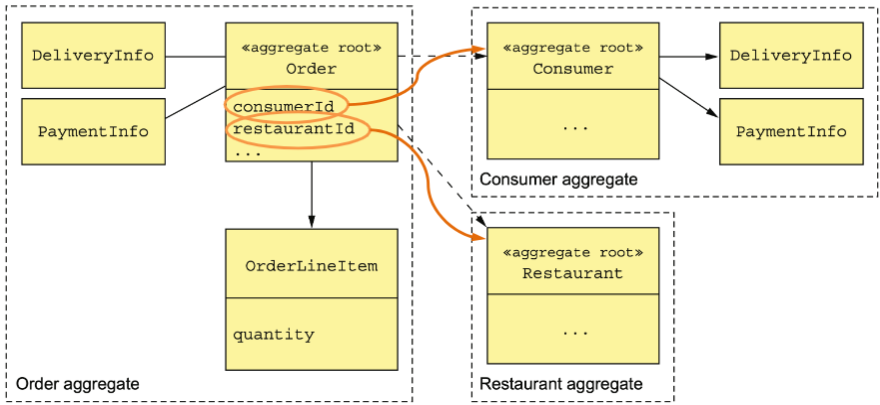
\includegraphics[width=\linewidth]{content/chapters/images/2026-04-11-13-03-08.png}
  \end{minipage}
\end{flushleft}



\begin{flushleft}
  \begin{minipage}{0.65\linewidth}
    \raggedright
    \subsection{Rule: one aggregate per transaction}
    One transaction operates on one
    aggregate only

    Consequences:
    \begin{itemize}
      \item Ensure a transaction is contained in a single service
      \item Suitable for limited transactions support in NoSQL databases
      \item Less efficient in transfer from/to db
      \item More complex implementation of complex requests that update multiple aggregates
    \end{itemize}
  \end{minipage}%
  \hfill
  \begin{minipage}{0.3\linewidth}
    \centering
    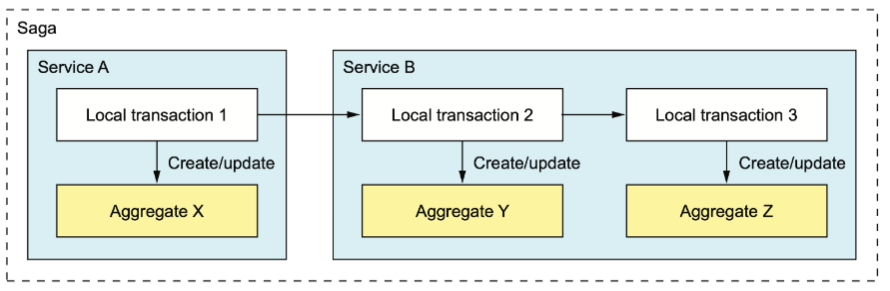
\includegraphics[width=\linewidth]{content/chapters/images/2026-04-11-13-05-06.png}
  \end{minipage}
\end{flushleft}


\begin{center}
  \begin{minipage}{0.65\linewidth}
    \section{Split monolith with aggregates}
    Transformation into aggregates can help
    splitting the monolith. Services can be extracted easily.
  \end{minipage}%
  \hfill
  \begin{minipage}{0.3\linewidth}
    \centering
    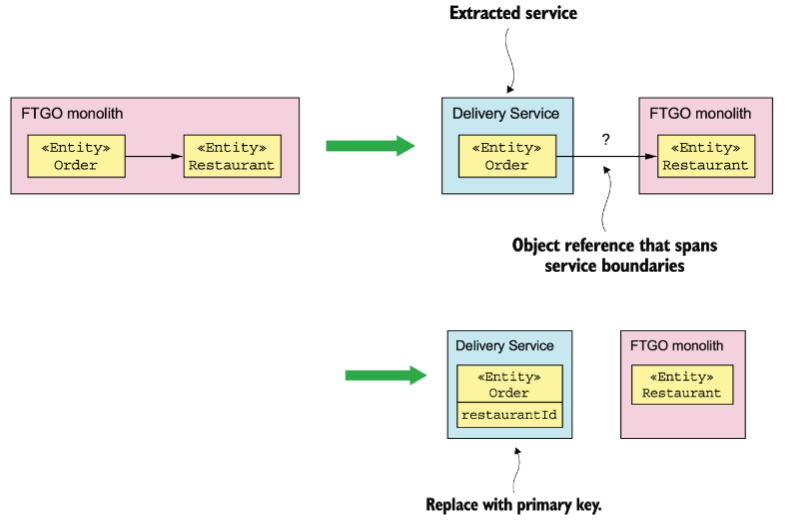
\includegraphics[width=\linewidth]{content/chapters/images/2026-04-11-13-06-23.png}
  \end{minipage}
\end{center}





\begin{flushleft}
  \begin{minipage}{0.65\linewidth}
    \raggedright
    \subsection{Aggregate granularity}

    \begin{itemize}
      \item Fine grained: Improve scalability (Updates on an aggregate are serialized), reduce the risk of conflicts and it is easier to decompose into services
      \item Coarse grained: More suitable to fit all relevant entities in a transaction
    \end{itemize}
  \end{minipage}%
  \hfill
  \begin{minipage}{0.3\linewidth}
    \centering
    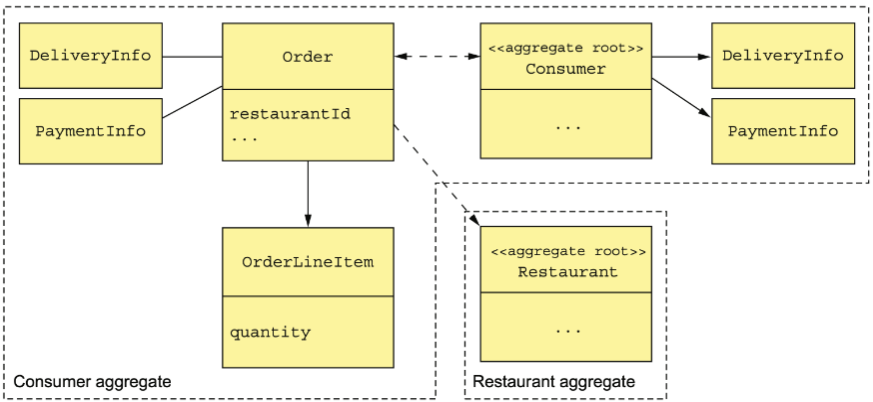
\includegraphics[width=\linewidth]{content/chapters/images/2026-04-11-13-19-09.png}
  \end{minipage}
\end{flushleft}


\subsection{Domain Events}


An Aggregate publishes a Domain Event when it's created or undergoes some other
significant change. Represented by a class in the domain model, the name is
formed using a past-participle verb phrase. E.g. \verb|OrderPlaced|, \verb|OrderShipped|, etc.

Properties that convey the event meaning. Each property is either a primitive value or a
value object, also metadata, e.g., event ID, timestamp

\begin{itemize}
  \item Maintaining data consistency across services
  \item Notifying a service that maintains a replica that the source data has changed
  \item Sending notifications to users
  \item Notifying another service to update related data
  \item Notifying a different application via a registered webhook or via a message broker
  \item Monitoring domain events to verify that the application is behaving correctly.
  \item Analyzing events to model user behavior
\end{itemize}


\section{Communication}



\begin{figure}[h!]
  \centering
  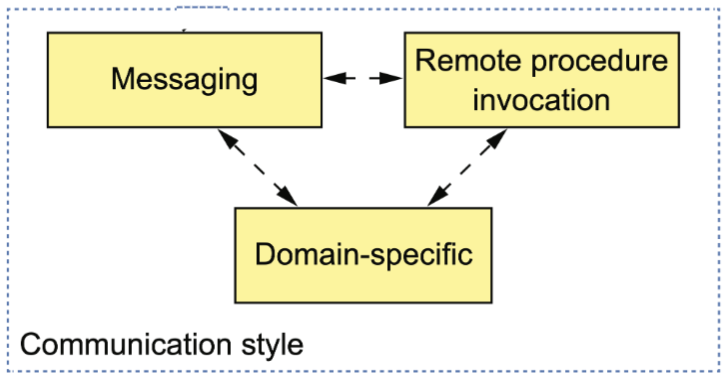
\includegraphics[width=0.4\linewidth]{content/chapters/images/2026-04-11-13-22-15.png}
\end{figure}


Ensure agreement on service interaction
mechanism to avoid late integration
issues:

\begin{itemize}
  \item Define the interface (using an IDL)
  \item Review with client services' developers
  \item Iterate to reach consensus
  \item Start implementation of services
\end{itemize}


\subsection{API evolution}

"An interactive software system must be
continually adapted or it becomes
progressively less satisfactory".

Aim for minor backward-compatible
changes.

Robustness principle:
\begin{itemize}
  \item Be conservative in what you do
  \item Be liberal in what you accept from others
\end{itemize}

\section{Message formats}

\begin{itemize}
  \item[] Text-based formats: JSON, XML, YAML
  \item[] Binary formats: Protocol Buffers, Avro, Thrift
\end{itemize}

Once the format is chosen, it might be mandated by the communication mechanism

\section{Remote procedure call (RPC)}


\begin{flushleft}
  \begin{minipage}{0.65\linewidth}
    \raggedright

    \begin{itemize}
      \item \textbf{Pros}: \textbf{Simple} and familiar, request-response is easy and the system is simple because of no intermediate broker
      \item \textbf{Cons}: Usually \textbf{only supports request/reply} and not other
            interaction patterns such as notifications, request/async response,
            publish/subscribe, publish/async response. \textbf{Reduced availability} since the client and the service
            must be available for the duration of the interaction
    \end{itemize}


    Requires service discovery

  \end{minipage}%
  \hfill
  \begin{minipage}{0.3\linewidth}
    \centering
    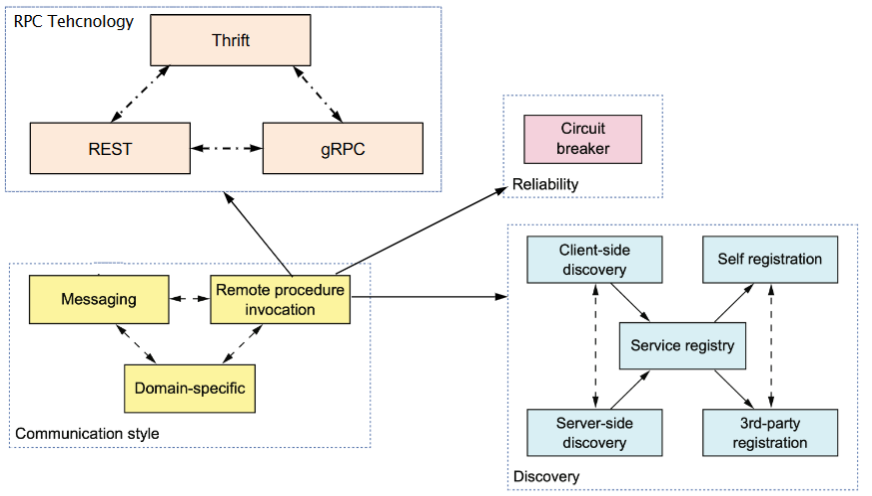
\includegraphics[width=\linewidth]{content/chapters/images/2026-04-11-13-26-20.png}
  \end{minipage}
\end{flushleft}


\subsection{Robust Synchronous APIs}

\begin{itemize}
  \item Network timeouts: Never block indefinitely, always use timeouts when
        waiting for a response
  \item Limit outstanding requests: Define an upper bound on the number of
        outstanding requests that a client can make to a particular service
  \item Circuit breaker pattern, allow failing fast
\end{itemize}

\subsection{Circuit Breaker pattern}

Service should be invoked through a proxy. Track the number of successful and failed
requests. If the error rate exceeds a threshold, trip the
circuit breaker so that further attempts fail
immediately. After a timeout period, the client should try again, and, if
successful, close the circuit breaker.

This is implemented by Netflix's Hystrix library.


\subsection{Service Discovery}

Using RPC you need to know the
network location of your service.


In microservices architectures service
instances change continuously due to:

\begin{itemize}
  \item Autoscaling
  \item Failures
  \item Updates
\end{itemize}



\begin{flushleft}
  \begin{minipage}{0.65\linewidth}
    \raggedright
    \subsubsection{Application level discovery}


    \begin{itemize}
      \item Self registration pattern: service register itself on activation and update list (Health check endpoint on server, Heartbeat API callback on registry)
      \item Client-side discovery pattern: Queries registry for active servers. Uses load balancing algorithm to pick one.
    \end{itemize}

  \end{minipage}%
  \hfill
  \begin{minipage}{0.3\linewidth}
    \centering
    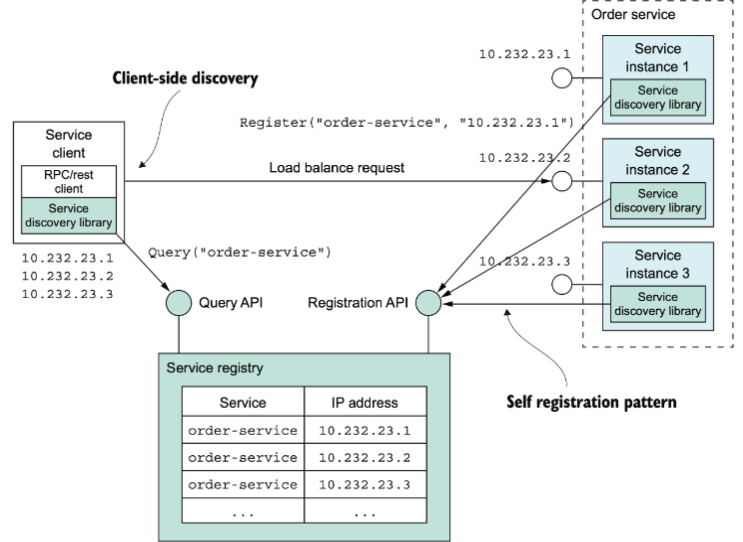
\includegraphics[width=\linewidth]{content/chapters/images/2026-04-11-13-35-30.png}
  \end{minipage}
\end{flushleft}



\begin{flushleft}
  \begin{minipage}{0.65\linewidth}
    \raggedright
    \subsubsection{Platform level discovery}

    \begin{itemize}
      \item Self registration pattern
      \item Third party registration pattern: Registrar component perform registration, often part of the platform (e.g., Kubernetes or Docker)
      \item Server-side discovery pattern: Client makes DNS request.
            Router access registry, load balance and resolve DNS
    \end{itemize}
  \end{minipage}%
  \hfill
  \begin{minipage}{0.3\linewidth}
    \centering
    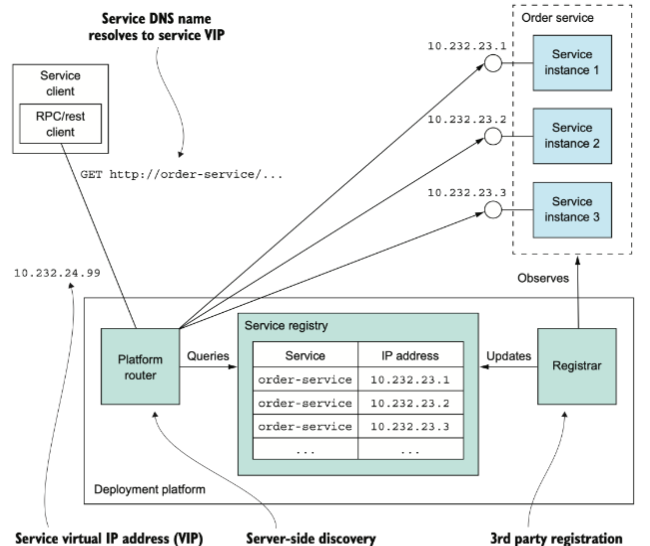
\includegraphics[width=\linewidth]{content/chapters/images/2026-04-11-13-35-54.png}
  \end{minipage}
\end{flushleft}




\section{Messaging}


\begin{flushleft}
  \begin{minipage}{0.65\linewidth}
    \raggedright
    \subsection{Competing receivers}

    \begin{itemize}
      \item Multiple receivers
      \item Each message must be processed only once or processed in order
      \item Sharded (partitioned) channels. The sender specifies a shard
            key in the message's header. The message broker uses a shard key to
            assign the message to a particular shard/partition.
    \end{itemize}

  \end{minipage}%
  \hfill
  \begin{minipage}{0.3\linewidth}
    \centering

    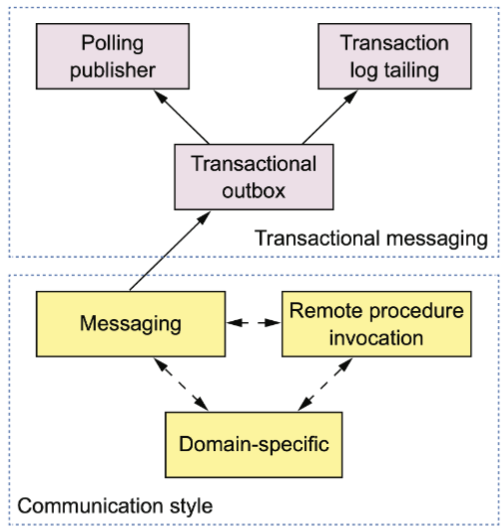
\includegraphics[width=\linewidth]{content/chapters/images/2026-04-11-13-47-31.png}
  \end{minipage}
\end{flushleft}




\section{Shared channels}

\begin{figure}[h!]
  \centering
  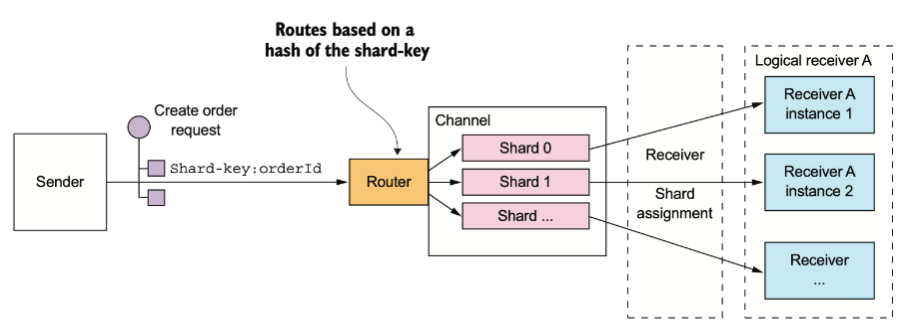
\includegraphics[width=0.4\linewidth]{content/chapters/images/2026-04-11-13-38-57.png}
\end{figure}


\subsection{Duplicate messages}
Failures of client, server, or broker might represent a problem. Message are guaranteed to be delivered at least once, but not only once. Possible countermeasures:
\begin{itemize}
  \item Idempotent messages
  \item Message tracking
\end{itemize}

\subsection{Transactional messaging}
Use a db table as a message queue. Keep in the same transaction:
\begin{itemize}
  \item Db application update
  \item Message queueing
\end{itemize}

\begin{flushleft}
  \begin{minipage}{0.65\linewidth}
    \raggedright
    \subsubsection{Transactional outbox}
    The outbox table acts as a message queue within the database.
    \begin{enumerate}
      \item The transaction updates the order table and inserts a message into the outbox table.
      \item A message relay reads the outbox table.
      \item The relay publishes the message to the message broker.
    \end{enumerate}
  \end{minipage}%
  \hfill
  \begin{minipage}{0.3\linewidth}
    \centering
    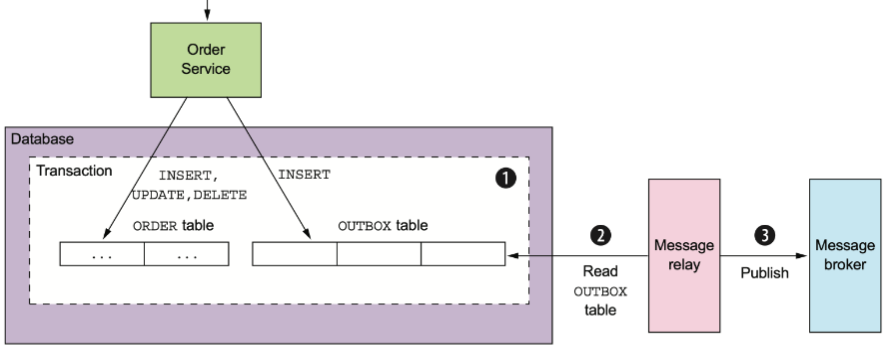
\includegraphics[width=\linewidth]{content/chapters/images/2026-04-11-14-00-14.png}
  \end{minipage}
\end{flushleft}



\begin{flushleft}
  \begin{minipage}{0.65\linewidth}
    \raggedright
    \section{Data and Transactions}

    \subsection{Database per service}
    Services must be loosely coupled so that they can be developed, deployed and scaled independently. Each service's persistent data is private and accessible only via its API, options:
    \begin{itemize}
      \item Private-tables-per-service
      \item Schema-per-service
      \item Database-server-per-service
    \end{itemize}
    A service's transactions only involve its db.

  \end{minipage}%
  \hfill
  \begin{minipage}{0.3\linewidth}
    \centering
    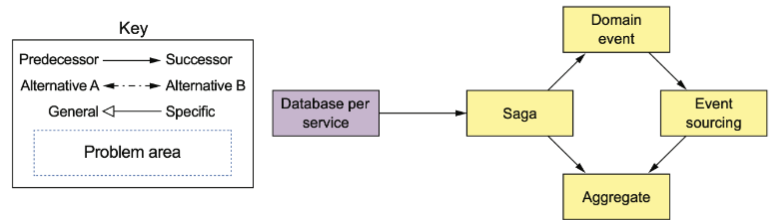
\includegraphics[width=\linewidth]{content/chapters/images/2026-04-11-14-00-42.png}
  \end{minipage}
\end{flushleft}





\subsection{Transactions in a monolith}
ACID db transaction : Atomicity, Consistency, Isolation, Durability.
Lack of isolation leads to:
\begin{itemize}
  \item Lost updates
  \item Dirty reads
  \item Nonrepeatable reads
\end{itemize}

\paragraph{Example: confirm order}
\begin{itemize}
  \item \textbf{Order Service:} Create an Order in an APPROVAL\_PENDING state.
  \item \textbf{Consumer Service:} Verify that the consumer can place an order.
  \item \textbf{Kitchen Service:} Validate order details and create a Ticket in the CREATE\_PENDING state.
  \item \textbf{Accounting Service:} Authorize consumer's credit card.
  \item \textbf{Kitchen Service:} Change the state of the Ticket to AWAITING\_ACCEPTANCE state.
  \item \textbf{Order Service:} Change the state of the Order to APPROVED state.
\end{itemize}

\subsection{Distributed data consistency}
\begin{itemize}
  \item \textbf{Distributed transaction - 2PC:} Query to commit, Agree/Abort, Commit/Rollback, Acknowledge.
  \item \textbf{Saga:} Local transactions coordinated with messages.
\end{itemize}

\subsubsection{Distributed transactions limits}
Transactions are not universally supported (e.g. NoSQL dbs, Modern message brokers). Transactions are synchronous, which means reduced availability. Isolation is overrated (most dbs adopt weaker isolation levels). Impossible to have both availability and most recent data.


\begin{center}
  \begin{minipage}{0.65\linewidth}
    \subsection{Saga pattern}
    A saga is a sequence of local transactions. Each local transaction updates the database and publishes a message or event to trigger the next local transaction in the saga. If a local transaction fails then the saga executes a series of compensating transactions (undo the changes that were made by the preceding local transactions).

  \end{minipage}%
  \hfill
  \begin{minipage}{0.3\linewidth}
    \centering
    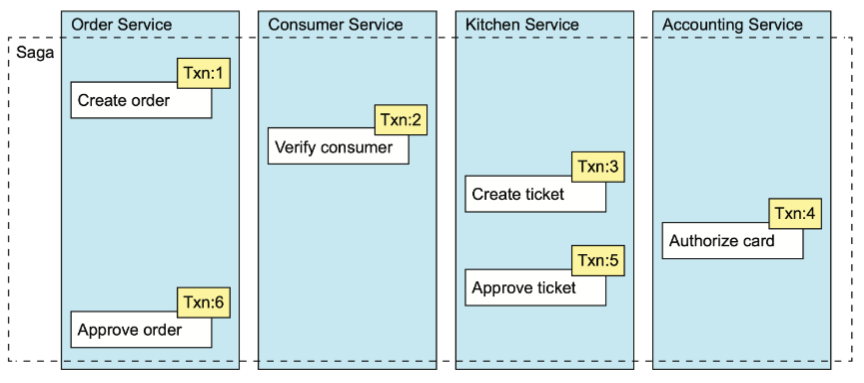
\includegraphics[width=\linewidth]{content/chapters/images/2026-04-11-14-01-16.png}
  \end{minipage}
\end{center}


\subsubsection{Compensating transactions}
Rollback is not directly supported since all service transactions are separate. Explicit invocation of compensating transactions in case of rollback (Used, e.g., when a check in a step fails).

\subsubsection{Saga transactions types}
\begin{itemize}
  \item \textbf{Compensatable transaction:} Can potentially be rolled back using a compensating transaction.
  \item \textbf{Pivot transaction:} The go/no-go point in a saga. If succeeds the saga can run until completion.
  \item \textbf{Retriable transaction:} Follow the pivot transaction and is guaranteed to succeed.
\end{itemize}

\subsubsection{Saga non-isolation}
\begin{itemize}
  \item \textbf{Atomic:} Managed by coordination mechanism and compensating transactions.
  \item \textbf{Consistent:} each service guarantee consistency in its own transaction.
  \item \textbf{Durable:} ensured by local db.
\end{itemize}
Non isolated problems: Lost updates, Dirty reads, Non-repeatable reads.

\subsubsection{Countermeasures for non-isolation}
\begin{itemize}
  \item \textbf{Semantic lock:} An application-level lock. A compensatable transaction sets a flag in any record that it creates or updates indicating it isn't fully committed. It's cleared by either a retriable transaction or a compensating transaction.
  \item \textbf{Commutative updates:} Design update operations to be executable in any order (e.g., \verb|Account.debit()| decrement balance).
  \item \textbf{Pessimistic view:} Reorder the steps of a saga to minimize business risk due to a dirty read.
        Cancel order (rolled back) and create order when executed concurrently could
        lead to exceeding customer's credit.
  \item \textbf{Reread value:} Prevent dirty writes by rereading data to verify that it's unchanged before overwriting it. If changed, saga aborts.
  \item \textbf{Version file:} Record the updates to a record so that they can be reordered (turns noncommutative operations into commutative).
  \item \textbf{By value:} Use each request's business risk to dynamically select the concurrency mechanism (sagas vs distributed transactions).
\end{itemize}

\subsection{Domain event pattern}
An aggregate publishes a domain event when it's created or undergoes some other significant change. A domain event is a class with properties that meaningfully convey the event, a name formed using a past-participle verb (e.g. \verb|OrderCreated|), and metadata (e.g. event ID, timestamp).

\subsection{Event sourcing}
Event sourcing is an event-centric technique for implementing business logic and persisting aggregates. An aggregate is stored in the database as a series of events, where each event represents a state change. It is an alternative to common persistence, e.g. through ORM.

\begin{table}[h!]
  \renewcommand{\arraystretch}{1.6}
  \centering
  \begin{tabularx}{0.8\textwidth}{X X}
    \toprule
    \textbf{Pros}                           & \textbf{Cons}                                                  \\
    \midrule
    Reliably publishes domain events        & It has a different programming model that has a learning curve \\
    Preserves the history of aggregates     & Messaging-based application are complex                        \\
    Avoids the O/R impedance mismatch       & Evolving events can be tricky                                  \\
    Provides developers with a time machine & Deleting data is tricky                                        \\
                                            & Querying the event store is challenging                        \\
    \bottomrule
  \end{tabularx}
\end{table}

\newpage
\section{Queries}

Queries can be Simple (require data from a single \(\mu\)S db) or Composed (required data from multiple \(\mu\)S dbs).

\begin{flushleft}
  \begin{minipage}{0.65\linewidth}
    \raggedright
    \subsection{API Composition}
    \begin{itemize}
      \item \textbf{API Composer:} Implement a query that retrieves data from several services by querying each service via its API and combining the results.
      \item \textbf{Provider Service:} Implement a service-limited query, limited by how data is partitioned and capabilities of APIs/databases.
    \end{itemize}
    Composer role can be Client (e.g. web app backend), API Gateway, or a Standalone service. For efficiency, parallelize queries as much as possible.
  \end{minipage}%
  \hfill
  \begin{minipage}{0.3\linewidth}
    \centering
    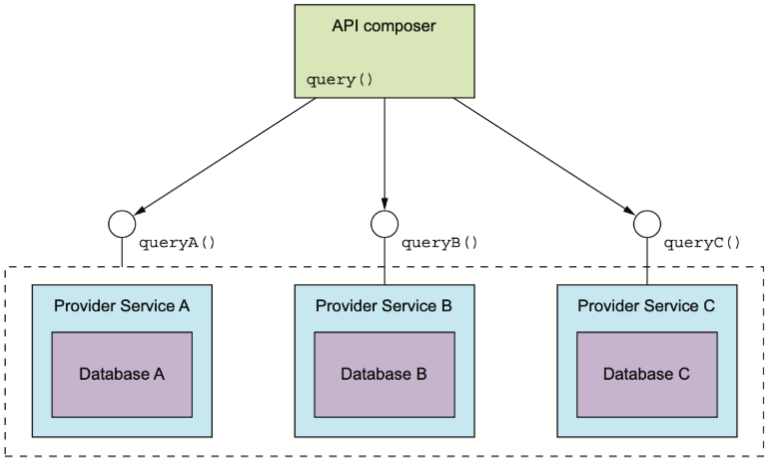
\includegraphics[width=\linewidth]{content/chapters/images/2026-04-11-14-01-58.png}
  \end{minipage}
\end{flushleft}



\begin{flushleft}
  \begin{minipage}{0.65\linewidth}
    \raggedright
    \subsection{CQRS}
    \textbf{C}ommand - \textbf{Q}uery \textbf{R}esponsibility \textbf{S}egregation.
    Use events to maintain a read-only view that replicates data from the services. The view can be easily queried.

    Design the schema to match the queries.
    The data access module must handle idempotent updates and concurrent updates.
    Implement a mechanism to efficiently build or rebuild the view, and cope with the replication lag.
  \end{minipage}%
  \hfill
  \begin{minipage}{0.3\linewidth}
    \centering
    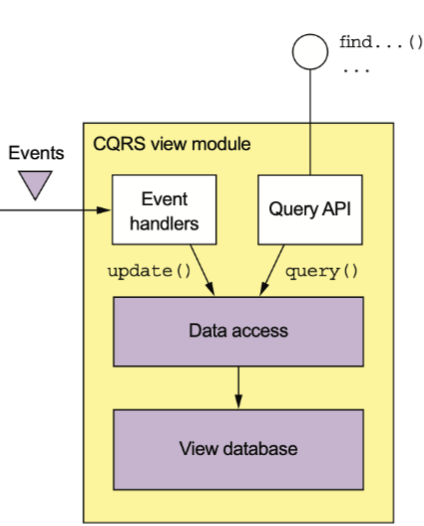
\includegraphics[width=0.65\linewidth]{content/chapters/images/2026-04-11-14-03-09.png}
  \end{minipage}
\end{flushleft}

\begin{figure}[h!]
  \centering
  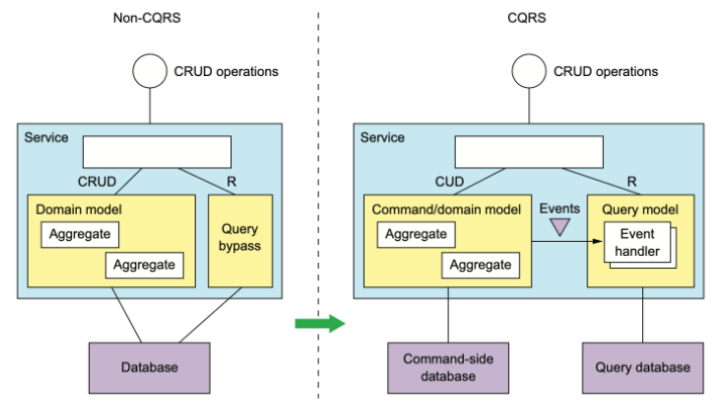
\includegraphics[width=0.45\linewidth]{content/chapters/images/2026-04-11-16-39-52.png}
\end{figure}


\section{External API}
External clients have low bandwidth (negative impact on UX) and lack of encapsulation. Different communication mechanisms are used.
Possible solutions:

\begin{center}
  \begin{minipage}{0.45\linewidth}
    \paragraph{Edge Functions} Authentication, Authorization, Rate limiting, Caching, Metrics collection, Request logging.

    \centering
    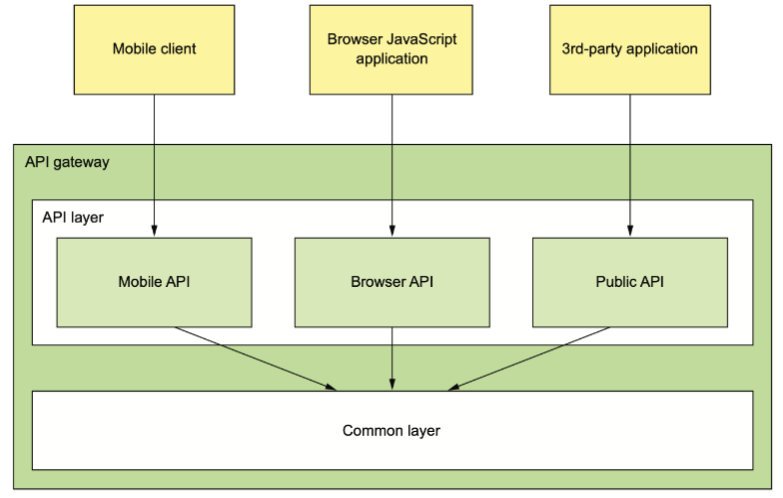
\includegraphics[width=0.4\linewidth]{content/chapters/images/2026-04-11-14-03-34.png}

  \end{minipage}%
  \hfill
  \begin{minipage}{0.45\linewidth}
    \paragraph{Backend for Frontend (BFF)}


    \centering
    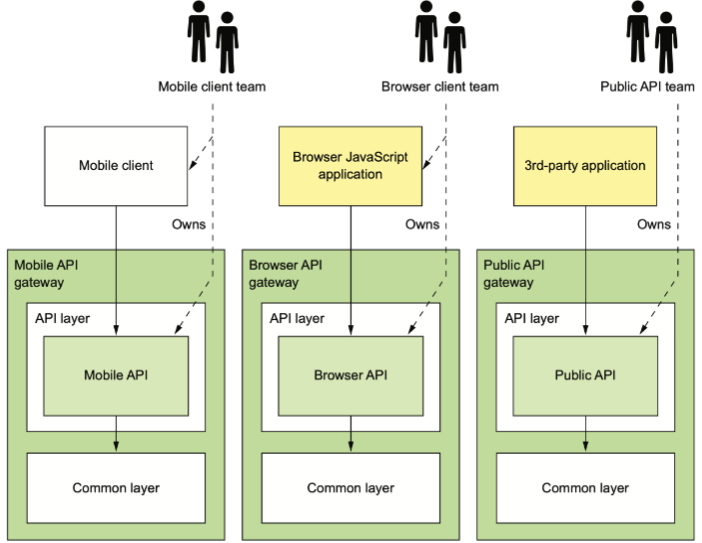
\includegraphics[width=0.4\linewidth]{content/chapters/images/2026-04-11-14-05-32.png}

  \end{minipage}
\end{center}


\section{Transition to Microservices}

\begin{itemize}
  \item \textbf{Big-bang rewrite:} "the only thing a Big Bang rewrite guarantees is a Big Bang!" (M.Fowler) .
  \item \textbf{Strangling the monolith:} Progressively wrap the monolith until it becomes an empty shell.
\end{itemize}

\begin{flushleft}
  \begin{minipage}{0.65\linewidth}
    \raggedright
    \subsection{Strangling the monolith}

    \textbf{Context}: a monolith application should be migrated to a micro service
    one

    \textbf{Problem}: a complete big-bang rewrite poses several risks

    \textbf{Solution:} gradually create a new system around the edges of the old, letting it grow slowly over several years until the old system is strangled.

    \textbf{Consequences:} Reduced risks, frequent releases allow to monitor the process and provide steady release of value, speed of transition can be adjusted.
  \end{minipage}%
  \hfill
  \begin{minipage}{0.3\linewidth}
    \centering
    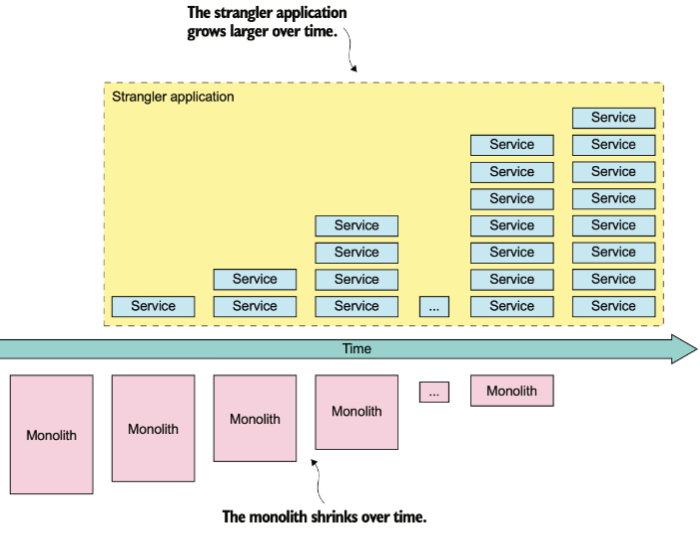
\includegraphics[width=\linewidth]{content/chapters/images/2026-04-11-14-06-47.png}
  \end{minipage}
\end{flushleft}


\subsection{Transition strategies}
\begin{itemize}
  \item \textbf{Implement new features as services:} Stop the growth of the monolith. API gateways reroute requests. Integration glue code integrates the service with the monolith (typically adapters).
  \item \textbf{Separate presentation and backend:} Represents an intermediate strategy.
  \item \textbf{Break up the monolith:} Extract functionalities into services. Extract a vertical slice (Inbound adapters, Domain logic, Outbound adapters, Monolith’s database schema).
\end{itemize}

\begin{center}
  \begin{minipage}{0.75\linewidth}
    \begin{minipage}[t]{0.45\linewidth}

      \centering
      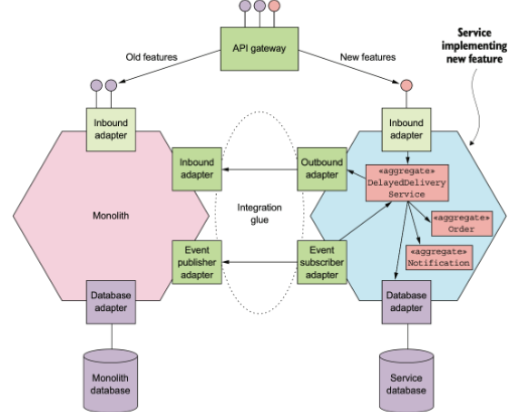
\includegraphics[width=\linewidth]{content/chapters/images/2026-04-11-16-46-51.png}
      \captionof{figure}{New features as services}
    \end{minipage}%
    \hfill
    \begin{minipage}[t]{0.45\linewidth}
      \centering
      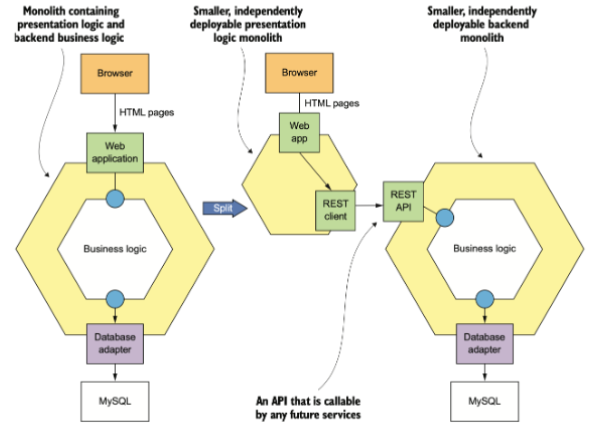
\includegraphics[width=\linewidth]{content/chapters/images/2026-04-11-16-47-38.png}
      \captionof{figure}{Split separation and backend}
    \end{minipage}
  \end{minipage}
\end{center}


\subsection{Refactor DB}
Several classes are persistent so the relative tables in the db must be refactored. Replicate data to avoid widespread changes in the monolith (Keep original schema and use triggers to update data).

\paragraph{Selecting services to migrate}
Rank modules by anticipated value your organization can get by migrating:
\begin{itemize}
  \item Features providing new business capabilities
  \item Accelerated development
  \item Performance, scaling, reliability issues
  \item Unlock migration of other more valuable modules
\end{itemize}

\begin{flushleft}
  \begin{minipage}{0.65\linewidth}
    \raggedright
    \subsection{God Class}
    An object that controls way too many other objects in the system and has grown beyond all logic to become The Class That Does Everything. Often implements business logic for many different aspects.

    \textbf{Splitting the God Class:} Apply DDD to separate domain models into subdomains. Avoid tight coupling among services and avoid a data service. Different views must be kept consistent (via Saga) and UX must be adapted to the set of partial models (via API gateway).
  \end{minipage}%
  \hfill
  \begin{minipage}{0.3\linewidth}
    \centering
    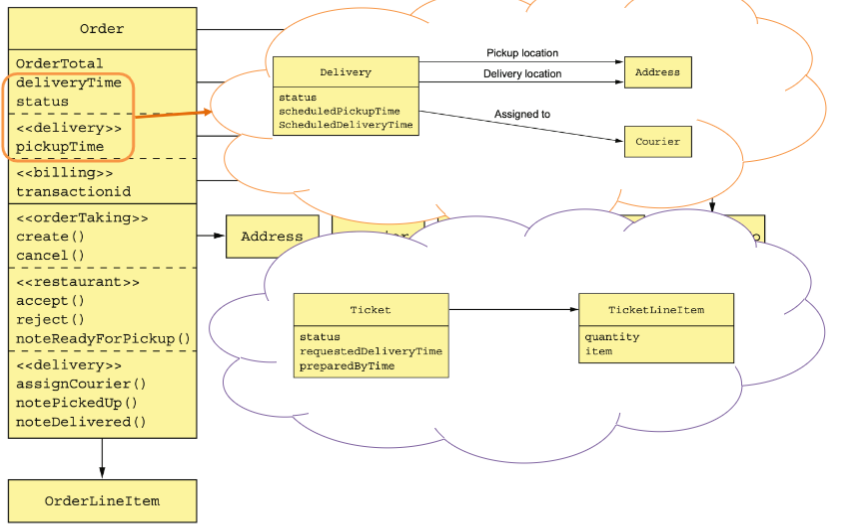
\includegraphics[width=\linewidth]{content/chapters/images/2026-04-11-14-09-36.png}
  \end{minipage}
\end{flushleft}

